\documentclass[handout]{beamer}

%%%%%%%%%%%%%%%%%%  PACKAGES %%%%%%%%%%%%%%%%%%
\usepackage{etex}
\usepackage{enumerate}
\usepackage{graphicx}
\usepackage{amsmath}
\usepackage{amssymb}
\usepackage{verbatim}
\usepackage{ifpdf}
\usepackage{bm}
\usepackage{ctable}
\usepackage{epstopdf}
\usepackage{graphicx}
\usepackage{graphics}
\usepackage[english]{babel}
\usepackage{bbm}
%\usetheme{Copenhagen}
%\usetheme{Singapore}
%\usetheme{Malmoe}
\usetheme{CambridgeUS}
%\usetheme{Amsterdam}
\usefonttheme{professionalfonts} % using non standard fonts for beamer
\usecolortheme{beaver}
%\usefonttheme{serif} % default family is serif
\usepackage{bbding}
\usepackage{color}
\usepackage{soul}
\usepackage{isaacshortcuts}
\usepackage{tikz}
\usetikzlibrary{decorations.pathreplacing}
\usetikzlibrary{trees}
%\DeclareMathSizes{5}{5}{5}{5}
%%%%%%%%%%%%%%%%%%  SHORTCUTS STUFF %%%%%%%%%%%%%%%%%%

\def\bi{\begin{itemize}}
\def\ei{\end{itemize}}
\def\ben{\begin{enumerate}}
\def\een{\end{enumerate}}
\def\i{\item [$\color{black}\bullet$]}
\def\bee{\begin{equation*}}
\def\eee{\end{equation*}}
\def\ba{\begin{eqnarray}}
\def\ea{\end{eqnarray}}
\def\baa{\begin{eqnarray*}}
\def\eaa{\end{eqnarray*}}
\def\bg{\beta}
\def\ag{\alpha}
\def\og{\omega}
\def\veg{\varepsilon}
\def\lf{\left}
\def\rg{\right}
\def\mc{\mathcal}
\def\td{\tilde}
\def\v{\vspace{0.2cm}}
\def\vv{\vspace{0.4cm}}




%%%%%%%%%%%%%%%%%%  SLIDES FORMATING %%%%%%%%%%%%%%%%%%
\setbeamertemplate{navigation symbols}{}
\setbeamertemplate{frametitle}[default][center]
\setbeamertemplate{footline}{%
\leavevmode%
\hbox{

%\begin{beamercolorbox}[wd=.25\paperwidth,ht=2.5ex,dp=1ex,center]{date in head/foot}%
%\usebeamerfont{date in head/foot}\insertshortdate
%\end{beamercolorbox}%
\begin{beamercolorbox}[wd=1\paperwidth,ht=2.5ex,dp=1ex,center]{title in head/foot}%
\usebeamerfont{title in head/foot}{F303 Intermediate Investments -  Isaac Hacamo}
\end{beamercolorbox}%
\begin{beamercolorbox}[wd=.25\paperwidth,ht=2.5ex,dp=1ex,center]{pages in head/foot}%
\usebeamerfont{pages in head/foot} \insertframenumber{} / \inserttotalframenumber\hspace*{2ex}
\end{beamercolorbox}

}
\vskip0pt%
}


\begin{document}

\title{\textbf{F303 Intermediate Investments}}
\author{Lecture 15: Stock Options \vspace{-1cm}}
\date{}
\frame[plain]{\titlepage}
\setcounter{framenumber}{0}


%%%%%%%%%%%%%%%%%%  SLIDE  %%%%%%%%%%%%%%%%%%
\frame{\frametitle{\large{\textbf{Goals for Today}}}
\bi
\i Finish problem from last lecture
\vv
\i Option trading.
\vv
\i Option contracts.
\vv
\i Calls and Puts.
\vv
\i Payoffs from Calls and Puts.
\vv
\ei
}

\frame{\frametitle{\large{\textbf{Review from Last Lecture: Duration}}}
Duration of a bond can be computed using the following:
\baa
D=1\times \frac{C/(1+y_1)}{Price}+2\times \frac{C/(1+y_2)^2}{Price}+\dots +T\times \frac{(F+C)/(1+y_T)^T}{Price}
\eaa
}


\frame{\frametitle{\large{\textbf{Review from Last Lecture: Bond Price Changes}}}
Bond price volatility is proportional to the bond's duration; therefore duration becomes a natural measure of interest rate exposure.
\baa
\frac{\Delta P}{P}=-D\times \frac{\Delta y}{1+y}
\eaa
where $y$= annual YTM and $D$= duration expressed in years. This formula is only valid for small changes in yields from the current level. It derives from a linearization of the bond price formula around the current yield.
}

\frame{\frametitle{\large{\textbf{Extra Comment on Duration: Convexity}}}
Bond prices are convex with respect to the yield to maturity. This is why large changes in yields will lead to larger changes in prices than the prediction from the result in the previous slide.
\begin{center}
\includegraphics[scale=0.5]{bod34698_11/bod34698_1105.jpg}
\end{center}
}

\frame{\frametitle{\large{\textbf{Extra Comment on Duration: Different Bonds}}}
How does the coupon rate affect the duration of a bond?
\begin{center}
\includegraphics[scale=0.5]{bod34698_11/bod34698_1102.jpg}
\end{center}
}


\frame[t]{\frametitle{\large{\textbf{Finish Problem from last lecture: Problem 1}}}
An investor has \$100,000 to invest. She borrows another \$80,000 by issuing 10-year zero coupon bonds worth \$80,000 today. She invests \$70,000 in 3-year zero coupon bonds and \$110,000 in a coupon bond with duration of 4 years. \\
\vv
a) What is the duration of her portfolio?\\

}

\frame[t]{\frametitle{\large{\textbf{Finish Problem from last lecture: Problem 1}}}
An investor has \$100,000 to invest. She borrows another \$80,000 by issuing 10-year zero coupon bonds worth \$80,000 today. She invests \$70,000 in 3-year zero coupon bonds and \$110,000 in a coupon bond with duration of 4 years. \\
\vv
a) What is the duration of her portfolio?\\

\color{red}
The total value of her portfolio is \$100,000 (=110k+70k-80k).
\baa
D_p&=&\frac{70}{100}\times 3 +\frac{110}{100}\times 4 -\frac{80}{100}\times 10=-1.5
\eaa
}

\frame[t]{\frametitle{\large{\textbf{Problem 1 (cont)}}}
b) The yield curve is currently flat at 4\%. If the yield curve shifts up by 0.5\% in a few days, will she have a gain or a loss? Calculate it in percent.
}

\frame[t]{\frametitle{\large{\textbf{Problem 1 (cont)}}}
b) The yield curve is currently flat at 4\%. If the yield curve shifts up by 0.5\% in a few days, will she have a gain or a loss? Calculate it in percent.
\color{red}
\baa
\frac{\Delta P}{P}&=&-D\times \frac{\Delta y}{1+y}\\
\frac{\Delta p}{p}&=&-(-1.5)\times \frac{0.005}{1+0.04}\\
&=&0.00721=0.721\%
\eaa
Because duration is negative an increase in yields leads to an increase in the value of the portfolio!
}

\frame[t]{\frametitle{\large{\textbf{Problem 1 (cont)}}}
c) Assume that she can choose the duration of the coupon bond. What bond duration should she pick to have a portfolio with no interest rate risk?\\
}

\frame[t]{\frametitle{\large{\textbf{Problem 1 (cont)}}}
c) Assume that she can choose the duration of the coupon bond. What bond duration should she pick to have a portfolio with no interest rate risk?\\
\color{red}
A bond has no interest rate risk if duration is equal to zero. We will use the formula for the duration of the portfolio and impose that the duration of the coupon bond is unknown, that is: 
\baa
D_p&=&\frac{70}{100}\times 3 +\frac{110}{100}\times D_c -\frac{80}{100}\times 10=0\\
\\
\rightarrow D_c&=&5.36\ \text{years}
\eaa

}

\frame[t]{\frametitle{\large{\textbf{Problem 1 (cont)}}}
d) Assume that she can borrow any amount (by issuing 10-year zero coupon bonds), and that she wants to invest an equal amount in the 3-year zero coupon bond and in the coupon bond with duration of 4 years. How much should she borrow to have a portfolio with no interest rate risk?\\
}

\frame[t]{\frametitle{\large{\textbf{Problem 1 (cont)}}}
d) Assume that she can borrow any amount, and that she wants to always invest an equal amount in the 3-year zero coupon bond and in the coupon bond with duration of 4 years. How much should she borrow to have a portfolio with no interest rate risk?\\
\color{red}

Here we also want to impose that the duration of the portfolio is  zero, but in this case we want to choose the amount to borrow, while imposing that the amount invested in the other two assets is always equal.
\baa
D=0&=&\frac{50+x/2}{100}\times 3 +\frac{50+x/2}{100}\times 4 -\frac{x}{100}\times 10\\
0&=&(50+x/2)\times 3 +(50+x/2)\times 4 -x\times 10\\
0&=&   350 -x\times 13/2\\
\rightarrow x&=&53,846.15
\eaa
}


%
%\frame[t]{\frametitle{\large{\textbf{Extra Practice Problems}}}
%\scriptsize
%\bi
%\i \ul{Problem 1}: You will be paying \$10k a year in tuition expenses at the end of the next two years. Assume that yield curve is flat and the yields are equal to 8\%.
%\bi
%\scriptsize
%\i What is the present value and duration of your obligation?
%\i What maturity zero-coupon bond would immunize your obligation?
%\i Suppose you buy a zero coupon bond with value and duration equal to your obligation. Now suppose that rates immediately increase to 9\%. What happens to your net position, that is, to the difference between the value of the bond and that your obligation? What is rates fall to 7\%?
%\ei
%\vv
%\i \ul{Problem 2}: You manage a pension fund that will provide retired workers with lifetime annuities. You determine that the payouts of the fund are essentially going to resemble level perpetuities of \$1 million per year. The interest rate is 10\%. You plan to fully fund the obligation using 5-year and 20-year maturity zero-coupon bonds.
%\bi
%\scriptsize
%\i How much market value of each of the zero coupon bonds will be necessary to fund the plan if you desire an immunization position?
%\i What must be the face value of the two zero coupon bonds to fund the plan?
%\ei
%\ei
%}


\frame{\frametitle{\large{\textbf{Derivative Instruments}}}
\begin{center}
Let's start a new part: \textbf{Options!}
\end{center}
}


\frame{\frametitle{\large{\textbf{Derivative Instruments}}}
\bi
\i A relatively recent, but extremely important class of financial assets is derivative securities.
\vv
\i These are securities whose values are determined by, or derived from� the prices of other securities.
\vv
\i These assets are also called contingent claims because their payoffs are contingent on other securities.
\vv
\i These assets are powerful tools for both hedging and speculation.
\ei
}

\frame{\frametitle{\large{\textbf{Example of Derivatives}}}
\bi
\i Call Option;
\vv
\i Put Options;
\vv
\i Swaps;
\vv
\i Futures;
\vv
\i Forwards;
\ei
Option contracts are traded now on several exchanges. They are written on common stock, stock indexes, foreign exchange, precious metals, interest rate futures, volatility
}


\frame{\frametitle{\large{\textbf{Option Contract}}}
\bi
\i \textbf{Call Option}
This is a right (but not an obligation) to buy an asset at a pre-arranged price (the \ul{exercise price} or \ul{strike price}) on or until a pre-arranged date (the \ul{maturity});
\vv
\i \textbf{Put Option}
This is a right (but not an obligation) to sell an asset at a pre-arranged price (the \ul{exercise price} or \ul{strike price}) on or until a pre-arranged date (the \ul{maturity}).
\ei
}


\frame{\frametitle{\large{\textbf{Call Options: Example}}}

\begin{center}
\footnotesize
Data from March 6th 2018 at 7.36pm
\vspace{0.5cm}
\includegraphics[scale=0.3]{./spy_2018_calls}
\end{center}
}


\frame{\frametitle{\large{\textbf{Put Options: Example}}}

\begin{center}
\footnotesize
Data from March 6th 2018 at 7.36pm
\vspace{0.5cm}
\includegraphics[scale=0.3]{./spy_2018_puts}
\end{center}
}



\frame{\frametitle{\large{\textbf{Call Option on S\&P 500: Example}}}
\begin{center}
\footnotesize
Data from March 6th 2018 at 7.36pm\\
\vspace{0.5cm}
\includegraphics[scale=0.3]{./spy_2018_call_price}\\
At the time when I got these prices, the SPY was trading at 272.83.
\end{center}
}


\frame{\frametitle{\large{\textbf{Call Options}}}
\bi
\i The purchase price of the option is called the premium. It is the compensation the purchaser of the call must pay for the right to exercise the option if exercise becomes profitable.
\vv
\i Sellers of the call option, who are said to write calls, receive premium income now as payment against the possibility they will be required at some later date to deliver the asset in return for an exercise price lower than the market value of the asset. 
\ei
}

\frame{\frametitle{\large{\textbf{Call Options: An Example}}}

\bi
\i Consider a call option on Priceline.com with an exercise price of \$1,760 per share that matures on March 31. On Friday, the right for that contract was \$8.97.
\vv
\begin{center}
\footnotesize
\includegraphics[scale=0.25]{./pcln_option_v2}
\end{center}
\i \ul{Let us say that on March 31, 2017, PCLN shares sell for \$1,721}. In this case, it does not make sense to exercise the option to buy at \$1,760, since you can buy PCLN for \$1,721 in the stock market.
\vv
\footnotesize
\i see all available options for Priceline.com at https://goo.gl/lRfJC9
\ei
}


\frame{\frametitle{\large{\textbf{Call Options: An Example}}}
\bi
\i If PCLN remains below \$1,760 until the expiration date, the call will expire worthless. 
\vv
\i If, on the other hand, the stock goes above \$1,760, the call holder will find it optimal to exercise. Why?
\vv
\i Let us say that at expiration, the shares trade at \$1,782. The option you bought allows you to buy a share of PCLN for \$1,760.  After exercising this option, you can then immediately turn around and sell your share for \$1,782 in the stock market!
\vv
\i The proceeds from exercise are given by:
Stock price - Exercise price = \$1,782 - \$1,760 = \$22
\ei
}


\frame{\frametitle{\large{\textbf{Payoff from Buying a Call Option}}}
\bi
\i When an investor \textbf{\ul{buys} a Call Option}, his payoff is equal to 
\baa
\text{Payoff}=\max\{0,S-X\},
\eaa
 where $X$ is the exercise price, and $S$ is the stock price.
\vv
\i If the stock price is higher than the strike price, the investor should exercise the option. His payoff will be $S-X$.
\vv
\i On the other hand, if the stock price is lower than the strike price, the investor should not exercise the option. His payoff will be zero!
\ei
}

\frame{\frametitle{\large{\textbf{Payoff from Buying a Call Option}}}
Graphical representation of the payoff and profit when an investor \textbf{\ul{buys} a Call Option}. 
\begin{center}
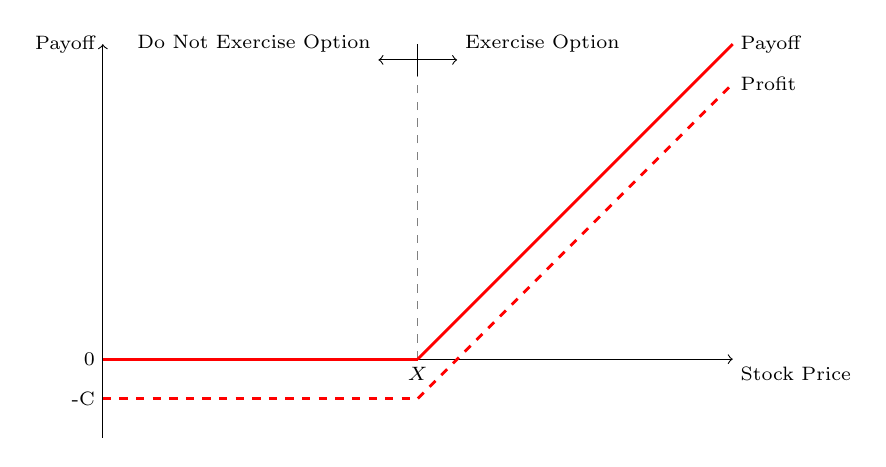
\begin{tikzpicture}
\scriptsize
\draw[->] (0,-1) -- (0,4);
\draw[->] (0,0) -- (8,0);
\draw[dashed,gray] (4,0) -- (4,4);
\draw[black] (4,3.6) -- (4,4);
\draw[->] (4,3.8) -- (4.5,3.8);
\draw (0,0) node[left] {0};
\draw (0,-0.5) node[left] {-C};
\draw (4.5,3.8) node[above right] {Exercise Option};
\draw (3.5,3.8) node[above left] {Do Not Exercise Option};
\draw[->] (4,3.8) -- (3.5,3.8);
%\draw[fill=black] (3,2.8) circle(0.1);
\draw (8,0) node[below right] {Stock Price};
\draw (0,4) node[ left] {Payoff};
\draw (4,0) node[below] {$X$};
\draw[line width=1pt,red] (0, 0) -- (4, 0);
\draw[line width=1pt,red] (4, 0) -- (8, 4);
\draw[dashed,line width=1pt,red] (0, -0.5) -- (4, -0.5);
\draw[dashed,line width=1pt,red] (4, -0.5) -- (8, 3.5);
\draw (8,4) node[right] {Payoff};
\draw (8,3.5) node[right] {Profit};
\end{tikzpicture}
\end{center}
$X$ is the exercise price, $S$ is the stock price, and $C$ is the price of the call option.
}


\frame{\frametitle{\large{\textbf{Payoff from Selling a Call Option}}}
\bi
\i When an investor \textbf{\ul{sells} a Call Option}, his payoff is equal to 
\baa
\text{Payoff}=-\max\{0,S-X\},
\eaa
 where $X$ is the exercise price, and $S$ is the stock price.
\vv
\i If the stock price is higher than the strike price, the investor should exercise the option. His payoff will be $-(S-X)$.
\vv
\i On the other hand, if the stock price is lower than the strike price, the investor should not exercise the option. His payoff will be zero!
\vv
\i When an investors sells a call option, he is on the other side of the trade. He profits if the option is not exercise, because he sold the option for $C$.
\ei
}

\frame{\frametitle{\large{\textbf{Payoff from Selling a Call Option}}}
Graphical representation of the payoff and profit when an investor \textbf{\ul{sells} a Call Option}. 
\begin{center}
\begin{tikzpicture}
\scriptsize
\draw[->] (0,-4) -- (0,1);
\draw[->] (0,0) -- (8,0);
\draw (0,0) node[left] {0};
\draw (0,0.5) node[left] {C};
%\draw[fill=black] (3,2.8) circle(0.1);
\draw (8,0) node[below right] {Stock Price};
\draw (0,1) node[ left] {Payoff};
\draw (4,0) node[above] {$X$};
\draw[line width=1pt,red] (0, 0) -- (4, 0);
\draw[line width=1pt,red] (4, 0) -- (8, -4);
\draw[dashed,line width=1pt,red] (0, 0.5) -- (4, 0.5);
\draw[dashed,line width=1pt,red] (4, 0.5) -- (8, -3.5);
\draw (8,-4) node[right] {Payoff};
\draw (8,-3.5) node[right] {Profit};
\end{tikzpicture}
\end{center}
$X$ is the exercise price, $S$ is the stock price, and $C$ is the price of the call option.
}


%
%\frame{\frametitle{\large{\textbf{Problem}}}
%What is the portfolio of calls and puts that provides the following payoff?
%\begin{center}
%\begin{tikzpicture}
%\scriptsize
%\draw[->] (0,-1) -- (0,4);
%\draw[->] (0,0) -- (8,0);
%\draw (0,0) node[left] {0};
%%\draw[fill=black] (3,2.8) circle(0.1);
%\draw (8,0) node[below right] {Stock Price};
%\draw (0,4) node[ left] {Payoff};
%\draw[line width=1pt,red] (0, 0) -- (2, 0);
%\draw (2, 0) node[below] {\$20};
%\draw[line width=1pt,red] (2, 0) -- (4, 2);
%\draw (0, 2) node[left] {\$20};
%\draw[line width=1pt,red] (4, 2) -- (6, 0);
%\draw (4, 0) node[below] {\$40};
%\draw[line width=1pt,red] (6, 0) -- (8, 0);
%\draw (6, 0) node[below] {\$60};
%\draw[dashed,gray] (4,0) -- (4,2);
%\draw[dashed,gray] (0,2) -- (4,2);
%\end{tikzpicture}
%\end{center}
%}
%
%
%\frame{\frametitle{\large{\textbf{Solution}}}
%\color{blue}
%You need to form the following portfolio:
%\bi
%\color{blue}
%\i Buy a call option with strike price of \$20
%\i Sell two call options with strike price of \$40
%\i Buy a call option with strike price of \$60
%\ei
%}
%

%%%%%%%%%%%%%%%%%%  SLIDE  %%%%%%%%%%%%%%%%%%

\newcounter{finalframe}
\setcounter{finalframe}{\value{framenumber}}

\setcounter{framenumber}{\value{finalframe}}
\end{document}


%%%%%%%%%%%%%%%%%  SLIDE  %%%%%%%%%%%%%%%%%%






